\documentclass{standalone}

\usepackage[compat=1.1.0]{tikz-feynman}

\begin{document}

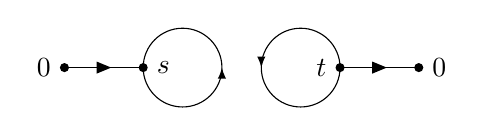
\begin{tikzpicture}

    \begin{feynman}[small]
        \vertex[dot, label=left:$0$] (x) {};
        \vertex[dot, right=of x, label=right:$s$] (a) {};
        \vertex[dot, right=2.5 of a, label=left:$t$] (b) {};
        \vertex[dot, right=of b, label=right:$0$] (y) {};

        \diagram* {
            (x) --[fermion] (a),
            (b) --[fermion] (y),
        };
    \end{feynman}

    \draw[
        decoration={markings, mark=at position 0 with {\arrow{latex}}},
        postaction={decorate}
    ]
    (a) ++ (0.5,0) circle (0.5);

    \draw[
        decoration={markings, mark=at position 0.5 with {\arrow{latex}}},
        postaction={decorate}
    ]
    (b) ++ (-0.5,0) circle (0.5);
\end{tikzpicture}

\end{document}